\documentclass[journal]{IEEEtran}
\usepackage{lipsum} % 示例中使用的假文宏包
\ifCLASSINFOpdf
\else
   \usepackage[dvips]{graphicx}
\fi
\usepackage{url}

\hyphenation{op-tical net-works semi-conduc-tor}
\usepackage{pdfpages} % 添加pdfpages宏包
\usepackage{graphicx}
\usepackage{xcolor}
\usepackage{amsmath}
\usepackage{listings}
\usepackage{matlab-prettifier}
\usepackage{float}
\usepackage{subfigure}

\definecolor{matlab_comment}{RGB}{28,172,0}
\definecolor{matlab_string}{RGB}{170,55,241}
\definecolor{matlab_keyword}{RGB}{0,0,255}
\definecolor{matlab_number}{RGB}{170,135,34}

\lstset{
    style=Matlab-editor,
    basicstyle={\fontsize{5}{5}\ttfamily},
    keywordstyle=\color{matlab_keyword},
    commentstyle=\color{matlab_comment},
    stringstyle=\color{matlab_string},
    numberstyle=\color{matlab_number},
    numbers=left,
    numbersep=-10pt,
    showspaces=false,
    showstringspaces=false,
}
\begin{document}
\title{\color[rgb]{0,0.6,1}Digital Signal Processing Course Laboratory Mini Project Report (November 2023)}

\author{12110405   Zhewei Chen}
%\thanks{This paragraph of the first footnote will contain the date on which you submitted your paper for review. It will also contain support information, including sponsor and financial support acknowledgment. For example, ``This work was supported in part by the U.S. Department of Commerce under Grant BS123456.'' }
%\thanks{The next few paragraphs should contain the authors' current affiliations, including current address and e-mail. For example, F. A. Author is with the National Institute of Standards and Technology, Boulder, CO 80305 USA (e-mail: author@boulder.nist.gov).}
%\thanks{S. B. Author, Jr., was with Rice University, Houston, TX 77005 USA. He is now with the Department of Physics, Colorado State University, Fort Collins, CO 80523 USA (e-mail: author@lamar.colostate.edu).}}

\markboth{EE323 Digital Signal Processing}
{Shell \MakeLowercase{\textit{et al.}}: Bare Demo of IEEEtran.cls for IEEE Journals}
\maketitle

\begin{abstract}
   This project displays how to convert sheet music into playable music 
   files using a computer program and explore how the fundamental elements of music 
   (pitch, rhythm, timbre, fundamental frequency, chords, etc.) are reflected in the data. 
   We implemented the conversion of sheet music to music data using MATLAB programming and 
   generated playable music and instrument imitations based on the data.
\end{abstract}

\begin{IEEEkeywords}
   music synthesis, MATLAB, numbered musical notation
\end{IEEEkeywords}


\IEEEpeerreviewmaketitle



\section{Introduction}
\IEEEPARstart{T}{his} project aims to explore the fundamental elements of music and implement the conversion of sheet music into playable music using MATLAB programming. In this project, we first introduce the basic elements of music, including pitch, rhythm, 
fundamental frequency, and chords. Then, we discuss how to reflect these musical elements in the data generated by a computer program. We represent numbered music notation as an M * N matrix, where N represents the number of channels, and each element represents the pitch or other musical elements at a specific time. Next, we use MATLAB programming to convert sheet music to music data. By writing a program, we can map the notes and rhythm information from the sheet music to the data matrix, thereby generating data that represents the music. Then, we use the built-in music playback functionality in MATLAB to convert the data into an audio signal and play it through speakers, ultimately saving it as an audio file. Furthermore, by studying the characteristics of specific instruments, we can adjust the details of the synthesizing music function program, such as the harmonic coefficients, to fit the sound of a particular instrument better. This experiment mainly focuses on the characteristics
 of the piano.






\section{Experimental Contents}
\label{sec:guidelines}


\subsection{Numbered Musical Notation}
\subsubsection{Tones}
$~$

In \textbf{numbered} musical notation, the numbers 1, 2, 3, 4, 5, 6, 7 (C, D, E, F, G, A, B) represent seven different pitches, which we refer to as tones. In the 12-tone equal temperament system, the frequency ratios between all the notes are equal, allowing us to calculate them using these multiples. By adding accidentals to the numbers 1-7  we can create 12 different pitches. Additionally, by using dots above or below the numbers, we can extend these pitches across multiple octaves. 

$~$

\textcolor[rgb]{0,0.6,1}{MATLAB practice 1:}

\begin{lstlisting}[style=Matlab-editor]
   function freq = tone2freq1(tone, noctave, rising)
\end{lstlisting}

Here, we are using three variables: "tone" to control the basic pitch level of 1-7 (with A4 at 440Hz ):
\begin{lstlisting}[style=Matlab-editor]
   ratio = [1 2^(1/6) 2^(1/6) 2^(1/12) 2^(1/6) 2^(1/6) 2^(1/6)];
   f = 440.* prod(ratio(1:tone));
\end{lstlisting}
 "noctave" to determine the number of octaves difference:
 \begin{lstlisting}[style=Matlab-editor]
   if noctave > 0
      f = f * 2*noctave;
   elseif noctave < 0
      f = f / (2*abs(noctave ));
   end
\end{lstlisting}
 "rising" to indicate whether the pitch is raised or lowered:
 \begin{lstlisting}[style=Matlab-editor]
   f = f * 2^(rising/12);
\end{lstlisting}
Then we can get the frequency of the tone when taking A4 (440 Hz) as the reference pitch.

\begin{figure}[htbp]
   \centering
   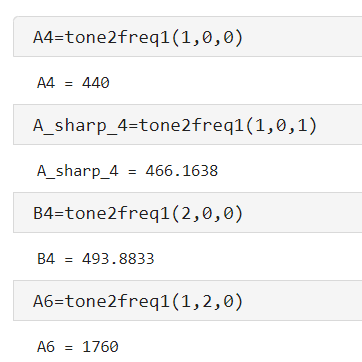
\includegraphics[width=0.44\textwidth]{p1.png} 
   \caption{Several tests for the function "tone2freq1"}
   \label{fig:1}
   \end{figure}

\subsubsection{Key Signatures}
$~~~~~~$

"Tones", "noctaves" and "rising" only represent the relative pitch of musical notes, so in numbered musical notation, we use key signature to determine the exact pitch of notes.
Then we make it possible to calculate the frequency of any note in a numbered musical notation.

$~$

\textcolor[rgb]{0,0.6,1}{MATLAB practice 2:}


\begin{lstlisting}[style=Matlab-editor]
   function freq = tone2freq(tone,scale, noctave, rising)
\end{lstlisting}


Based on tone2freq1, we add a new variable "scale" to determine the key signature of the music.
\begin{lstlisting}[style=Matlab-editor]
   % Define the base frequencies for each scale
   tone_list = [261.5 293.5 329.5 349 391.5 440 494];
   f = tone_list(scale) * prod(ratio(1:tone));
\end{lstlisting}

Then we can get the frequency of any tone of a numbered musical notation.
\subsection{Generate waveforms of different frequencies}



In MATLAB, generating waveforms of a specific frequency usually uses trigonometric functions.

We can write the frequency that we generated into trigonometric functions and play it using $sound$ function in MATLAB In music, there is also an important piece of information called \textcolor[rgb]{0,0.6,1}{rhythm}. We can achieve rhythm by adjusting the duration of each note. By programming, we can convert each note in the numeric notation into a musical scale represented by numbers 1 to 7. Then, by combining the duration of each note, we can generate the corresponding waveform for each note.

$~$

\textcolor[rgb]{0,0.6,1}{MATLAB practice 3:}

\begin{lstlisting}[style=Matlab-editor]
   function waves= gen_wave(tone,scale,noctave,rising,rhythm,fs)
\end{lstlisting}

The sampling frequency "fs" affects the accuracy and quality of music signal. Here we set it to 44100 Hz.This sampling frequency is sufficient to capture the frequency range that is perceptible to the human ear (up to approximately 20 kHz, which is the upper limit of human hearing).

Based on practice 1 and 2, we add the variable "rhythm" to determine the duration of each note.

\begin{lstlisting}[style=Matlab-editor]
   t = linspace(0, rhythm, fs * rhythm);
   o_mega = 2 * pi * f;
   waves=sin(o_mega*t);
\end{lstlisting}

After generating the waves of tones, we can combine them to generate the whole music.

\begin{lstlisting}[style=Matlab-editor]
   function music_sequence = gen_music(scale, fs,sequence,T)
   music_sequence = [];
   % gen_wave(tone,scale,noctave,rising,rhythm,fs)    
   [numRows, ~] = size(sequence);
      for row = 1:numRows
         rhythm = sequence(row, 4);
         rhythm=rhythm.*T;
         tone = sequence(row, 1);
         noctave= sequence(row, 2); 
         rising = sequence(row, 3);     
         wave = gen_wave(tone,scale,noctave,rising,rhythm,fs);
         music_sequence = [music_sequence, wave];
      end
   end
\end{lstlisting}

Because the "scale", "fs" is same for the same numbered musical notation, we only need to input the four variables.

Finally we can play and save the whole music.
\begin{lstlisting}[style=Matlab-editor]
   clc,clear,close all;
   scale=1;T=0.5;fs=44100;
   sequence1 = readmatrix('music.txt');
   %sequence =[tone noctave rsing rhythm]
   music=gen_music(scale,fs,sequence1,T);
   sound(music,fs)
   audiowrite("filename.wav",music,fs)
\end{lstlisting}
\subsection{Volume fluctuations}
Considering the decay of vibrations during instrument playing, where oscillations do not sustain at a fixed amplitude, an envelope decay function can provide a more realistic simulation of music production.

$~$

\textcolor[rgb]{0,0.6,1}{MATLAB practice 4:}
\begin{lstlisting}[style=Matlab-editor]
   waves = waves.* decay;
\end{lstlisting}

In addition to comparing them audibly, we also plotted the real waveform of a piano at the corresponding frequency for comparison.
We change the decay rate to select one that the waveform is most similar to the real waveform of a piano.

Fisrtly, we try to generate a simple exponential decay function. 
\begin{lstlisting}[style=Matlab-editor]
   %Exponential decay function
   decay_rate = 9; 
   decay = exp(-decay_rate * t / rhythm);
\end{lstlisting}
\begin{figure}[htbp]
   \centering
   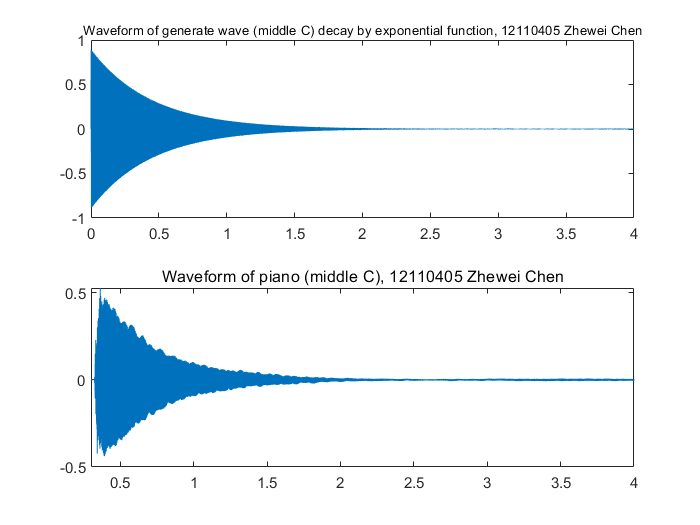
\includegraphics[width=0.52\textwidth]{p2.png} 
   \caption{Waveform with exponential decay function}
   \label{fig:2}
   \end{figure}
\begin{lstlisting}[style=Matlab-editor]
   % Linear deacy function
   decay_rate = 1/rhythm;
   decay =1-decay_rate*t;
   \end{lstlisting}
   \begin{figure}[htbp]
      \centering
      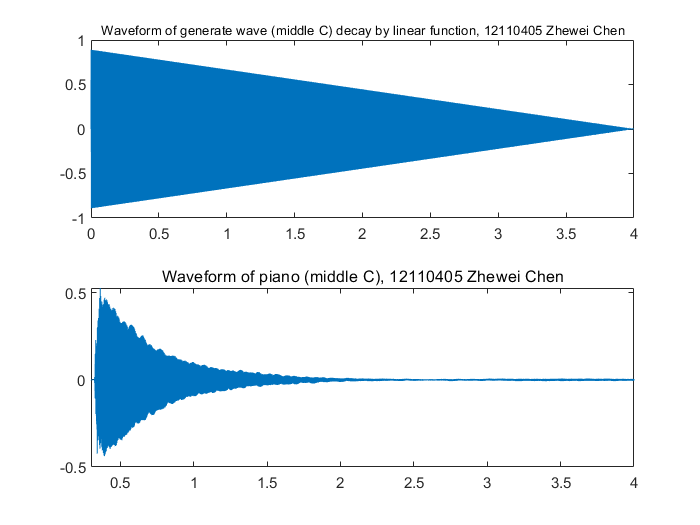
\includegraphics[width=0.52\textwidth]{p3.png} 
      \caption{Waveform with linear decay function}
      \label{fig:3}
      \end{figure}
   
\begin{lstlisting}[style=Matlab-editor]
   %Power exponential decay function
   decay_rate=9;
   r = 1/rhythm;  
   decay = (1 - r * t).^decay_rate; 
   \end{lstlisting}

Clearly, the waveform with power exponential decay function and exponential decay function are similar to the real waveform of a piano, while the waveform with linear decay function is not.


\begin{figure}[htbp]
   \centering
   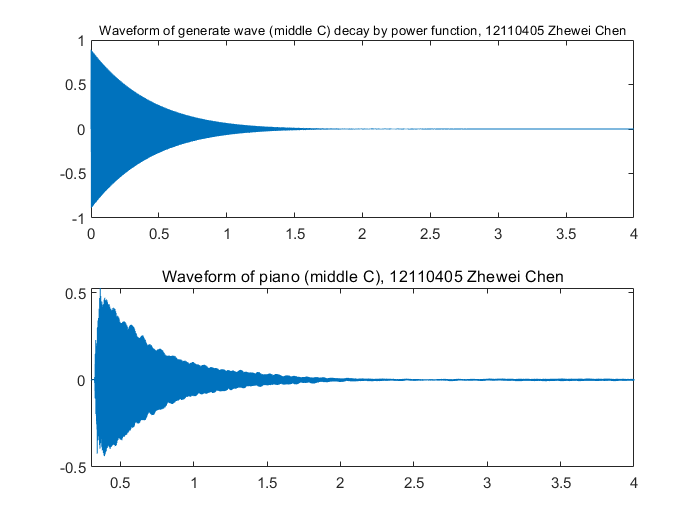
\includegraphics[width=0.52\textwidth]{p4.png} 
   \caption{Waveform with power exponential decay function}
   \label{fig:4}
   \end{figure}
   Nevertheless, 
   when we play the music with the $decay\_rate$ of 9 and decay function of exponential decay function, 
   the sound is too short and does not match the real music scene. We have adjusted the $decay\_rate$ to 3 after playing the music many times.


\subsection{Harmonics and timbre of instruments}
When playing a instrument, harmonics are generated, including the fundamental frequency and several integer multiples of that frequency. The main energy is concentrated in the fundamental frequency. The energy ratio of harmonics at 2 times, 3 times, 4 times, 5 times, and so on, varies for different musical instruments. If we adjust this ratio, it will produce completely different timbre of the sound wave.

Also changing the basic function of waves can generate different timbre of the sound wave.

$~$

\textcolor[rgb]{0,0.6,1}{MATLAB practice 5:}

$~$

\subsubsection{Different coefficients of harmonics}


$~$

Based on practice 3, we add the variable "coefficients" to determine the energy ratio of harmonics.

\begin{lstlisting}[style=Matlab-editor]
   % coefficients and frequencies of harmonics
   coefficients = [1, 0.1856, 0.1056, 0.0523, 0.0315, 0.0379]; 
   frequencies = [1, 2, 3, 4, 5, 6]; 
   values = sin(o_mega * frequencies' * t); 
   waves = coefficients * values; 
\end{lstlisting}

By performing the Fourier transform on each note of a piano and then applying the inverse Fourier transform, we discover that the harmonic coefficients, for different notes of the piano are distinct.
\begin{lstlisting}[style=Matlab-editor]
   for k=1:88
   filename = strcat(num2str(k),'.m4a'); 
   [y, fs] = audioread(filename);
   t = linspace(0, length(y)/fs, length(y));
   Y = fft(y);L = length(y);f = fs*(0:(L/2))/L;P = abs(Y/L);
   figure
   plot(f, P(1:L/2+1))
   if k<30
   xlim([0,3500])
   else
   xlim([300,6000])
   end
   title('Spectrum of piano, 12110405 Zhewei Chen')
   xlabel('frequency')
   ylabel('magnitude')
   fi = strcat(num2str(k), '.png');
   saveas(gcf, fi, 'png');
   end
\end{lstlisting}

After obtaining the spectrum, we observed a certain pattern in the coefficient distribution. As the piano frequency decreases, the coefficients of higher multiples of standing waves become larger, while as the frequency increases, the coefficients of the fundamental frequency become larger.

Based on the mainly frequency distribution of the chosen piece, I gradually adjusted the coefficients and made further refinements based on the actual perception of sound.

\begin{figure}[htbp]
   \centering
   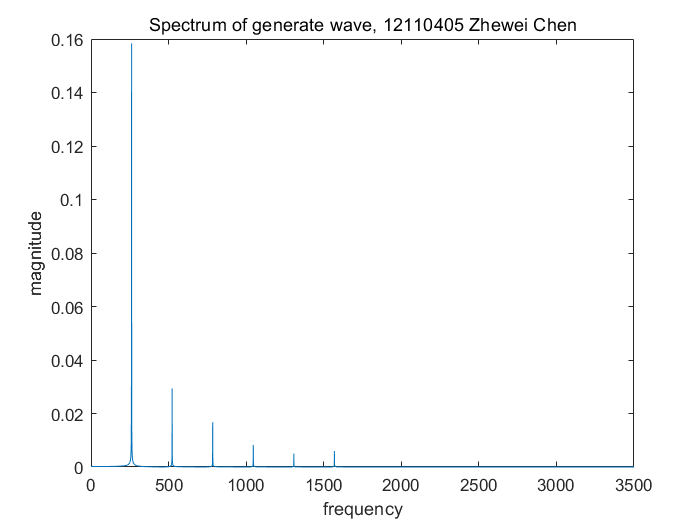
\includegraphics[width=0.42\textwidth]{m.png} 
   \caption{Waveform with basic function sawtooth}
   \label{fig:4}
\end{figure}
\begin{figure}[htbp]
   \centering
   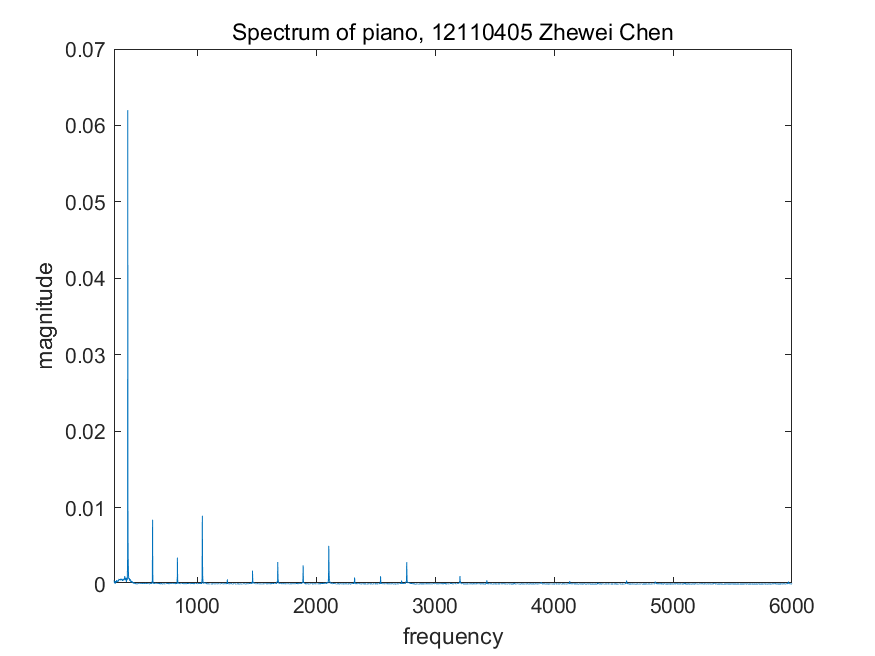
\includegraphics[width=0.43\textwidth]{36.png} 
   \caption{Waveform with basic function sawtooth}
   \label{fig:4}
\end{figure}


\subsubsection{Different basic function of waves}

$~$
\begin{lstlisting}[style=Matlab-editor]
   values = sin(o_mega * frequencies' * t); 
   % values = sawtooth(o_mega * frequencies' * t); 
   % values = square(o_mega * frequencies' * t);
   \end{lstlisting}

\begin{figure}[htbp]
   \centering
   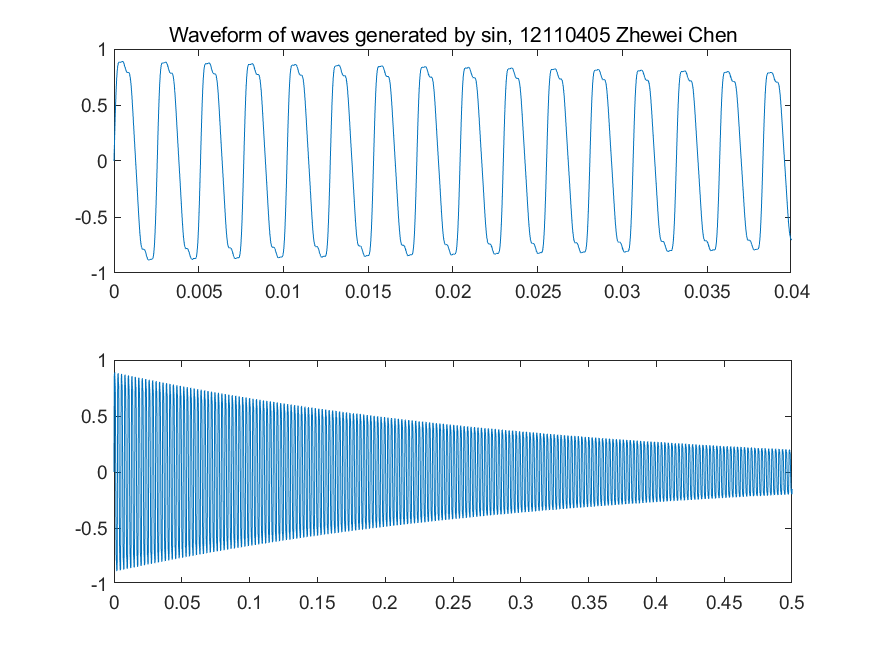
\includegraphics[width=0.5\textwidth]{1.png} 
   \caption{Waveform with basic function sin}
   \label{fig:4}
\end{figure}


\begin{figure}[htbp]
   \centering
   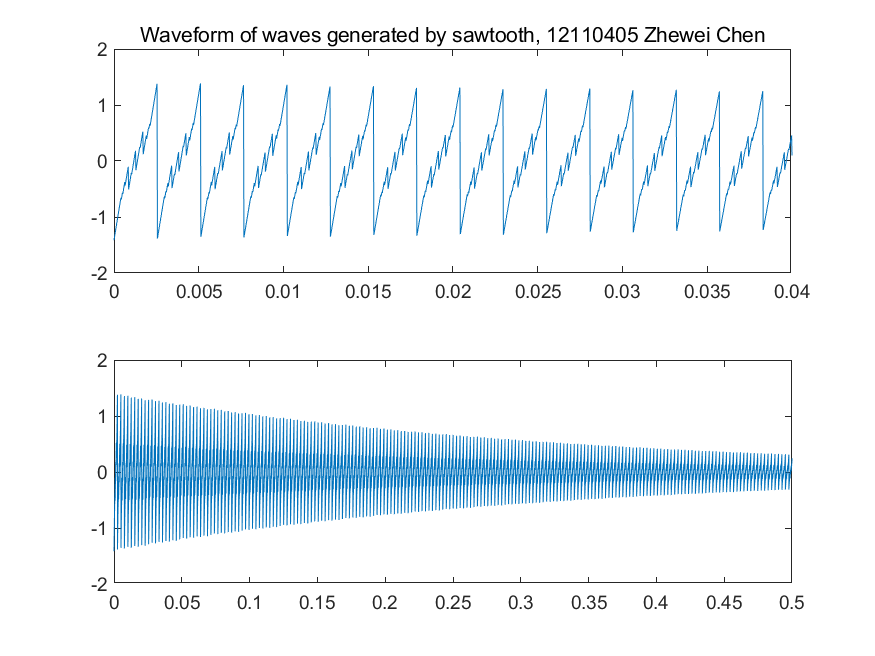
\includegraphics[width=0.5\textwidth]{2.png} 
   \caption{Waveform with basic function sawtooth}
   \label{fig:4}
\end{figure}


\begin{figure}[htbp]
   \centering
   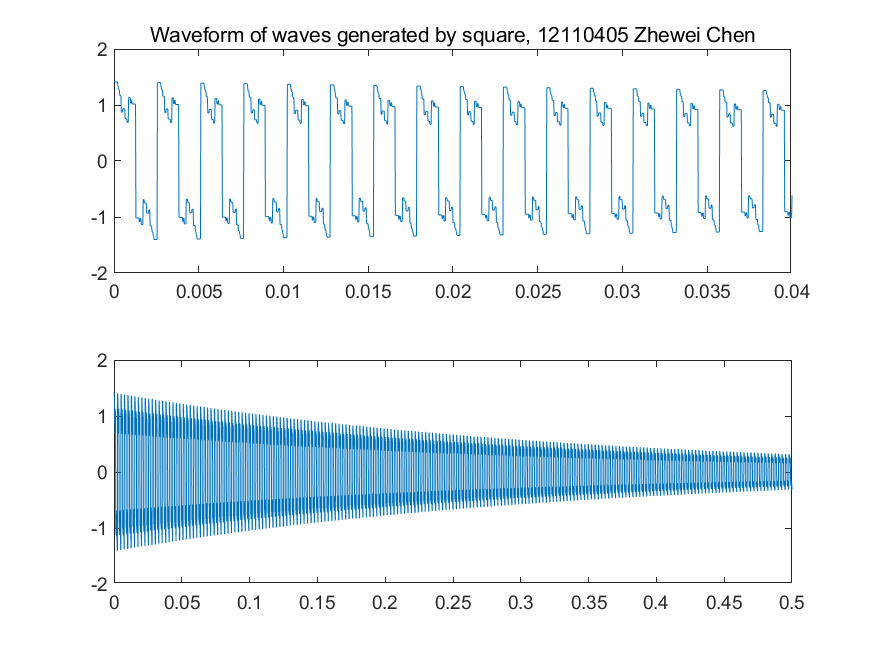
\includegraphics[width=0.5\textwidth]{3.png} 
   \caption{Waveform with basic function square}
   \label{fig:4}
\end{figure}
From the waveform, it can be observed that square waves and sawtooth waves exhibit larger fluctuations in amplitude, while sine waves appear smoother. In terms of auditory perception, sawtooth waves and square waves, especially sawtooth waves, have a distinct electronic sound and are more noisy, whereas sine waves sound clearer and more crisp.
\subsubsection{Different parts of the music}
The vast majority of music is played with different parts, including high and low parts. We can use different channels to play the prats simltaneously.

\begin{lstlisting}[style=Matlab-editor]
   sequence1 = readmatrix('.txt');
   %sequence =[tone noctave rsing rhythm]
   music=gen_music(scale,fs,sequence1,T);
   sequence2 = readmatrix('.txt');
  music1=gen_music(scale,fs,sequence2,T);
   combined_music = [music; music1];
   sound(combined_music,fs)
\end{lstlisting}
\section{Conclusion}
Through this experiment, we researched the process of converting musical notation into music using MATLAB. When simulating music, we first restored the corresponding notes and rhythm using the equal temperament tuning system. Then, we focused on recreating the timbre of the instrument. By comparing the sound perception and waveforms, we selected different basic waveform functions, harmonic coefficients, and decay functions to simulate the timbre of a particular instrument better. Additionally, we discovered that real music is more complex. For example, the decay of piano sounds is often intricate, and there are distinctions between sustained notes and staccato notes.

\end{document}
